\documentclass[compress]{beamer}
\usepackage{graphicx}
\usepackage{enumerate}
\usepackage[utf8]{inputenc}
\usepackage[T1]{fontenc}
\usepackage[francais]{babel}
\setbeamertemplate{caption}[numbered]
\title{Introduction à Git}
\author{Guillaume \textsc{Huysmans}}
\bibliographystyle{plain}
\newenvironment{envie}
	{\begin{block}{Ce qu'on a envie de dire...}}
	{\end{block}}
\newenvironment{curieux}
	{\begin{block}{Pour les curieux...}}
	{\end{block}}
\begin{document}
\begin{frame}
	\maketitle
\end{frame}
\begin{frame}
	\frametitle{Plan}
	\tableofcontents
\end{frame}


\section{Problématique}
\begin{frame}
	\frametitle{Collaboration}
	Un jour ou l'autre, on aura un projet à faire à plusieurs.
	Il devient nécessaire de fusionner les changements et de se synchroniser.

	\begin{envie}
	C'est faisable manuellement ! \pause
	\end{envie}

	\begin{itemize}
		\item par e-mail / réseau social \pause (trop volumineux ?) \pause
		\item par clé USB \pause (copier quoi ? dans quel sens ?) \pause
		\item à la Google Docs \pause (et sans connexion ?) \pause
		\item par un Drive quelconque \pause (conflits ?)
	\end{itemize}
\end{frame}

\begin{frame}
	\frametitle{Un bon contrôle de versions}
	\begin{itemize}
		\item Synchronisation (semi-)automatique
		\item Travail hors-ligne
		\item Décentralisé : pas d'obligation à utiliser un unique serveur
		\item Rapide (et cross-platform : GNU/Linux, Windows, OS X)
		\item Historisé :
			\begin{itemize}
				\item Liste lisible des derniers changements
				\item Qui a fait quoi ?
				\item Possibilité de revenir en arrière
			\end{itemize}
	\end{itemize}
\end{frame}


\section{Solution}
\begin{frame}
	\center
	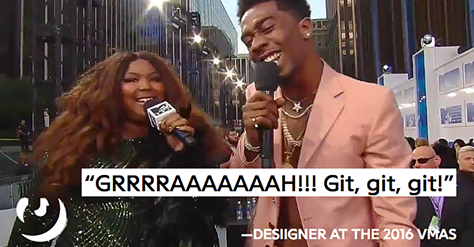
\includegraphics[width=\textwidth]{git-desiigner.png}
\end{frame}
\begin{frame}
	\frametitle{Git}
	Selon les critères précédents, Git,
	développé par Linus Torvalds (créateur de Linux),
	est un bon système de contrôle de versions. %(VCS en angais).

	\begin{itemize}
		\item Utilisations : \pause
			\begin{itemize}
				\item Le noyau Linux :
					\begin{itemize}
						\item Plus de 18 millions de lignes
						\item 91 Mo de texte compressé ! \pause
					\end{itemize}
				\item Des cours et manuels collaboratifs (à la Wiki) \pause
				\item \url{https://github.com/steeve/france.code-civil} \pause
			\end{itemize}
		\item Hébergement connu : \url{https://github.com} \pause
		\item Interfaces graphiques \pause
		\item Gère avant tout du texte (gênant ?)
	\end{itemize}
\end{frame}

\begin{frame}
	\frametitle{Du texte ?!}
	Le code source d'un programme est \emph{déjà} du texte.
	\pause

	Les documents peuvent aussi en être : il suffit de les rédiger en
	\LaTeX{} (comme cette présentation), Markdown... !
	\pause

	\begin{envie}
		Qu'est-ce qu'on y gagne ? \pause
	\end{envie}

	Avantages :
	\begin{itemize}
		\item Fusion parfois automatique des changements \pause
		\item Reproductibilité : le résultat sera le même partout. \pause
			\begin{itemize}
				\item La fusion n'est faite qu'une fois. \pause
				\item \LaTeX{} n'a pas autant de fantaisie que Word.
			\end{itemize}
	\end{itemize}
\end{frame}

\begin{frame}
	\frametitle{\LaTeX{} en un slide}
	Avantages :
	\begin{itemize}
		\item Transforme des instructions (texte) en un PDF
		\item Gratuit, fonctionne partout
		\item Programmable (langage Turing-complet) :
			possible d'ajouter des fonctionnalités
			(cohérence, graphiques, etc.)
	\end{itemize}
	Inconvénients :
	\begin{itemize}
		\item Langage pas très joli, un peu limité
		\item Pas facile à apprendre totalement
			\begin{itemize}
				\item Généralement pas nécessaire : il y a assez d'exemples !
			\end{itemize}
	\end{itemize}
\end{frame}

\begin{frame}
	\frametitle{Fonctionnement général}
	\begin{itemize}
		\item Toutes les versions sont archivées (sans doublons) \pause
		\item Les différences sont calculées à la demande. \pause
		\item Un ensemble cohérent de changements = un \emph{commit}. \pause
		\item Pour nous aider, un commit a :
			\begin{itemize}
				\item un titre
				\item une courte description (pas obligatoire) \pause
				\item un auteur
				\item une date \pause
			\end{itemize}
		\item Tout* commit a au moins un parent : celui qu'il a modifié. \pause
		\item Git retient à quelle version on est à travers des branches.
			\begin{itemize}
				\item Une branche contient l'empreinte de son dernier commit
					\pause
				\item Une branche avance avec les changements qu'on y fait.
					\pause
				\item On travaille directement sur les fichiers !
					\pause
			\end{itemize}
		\item Par défaut, tout se fait hors-ligne
			(\texttt{pull}/\texttt{push} manuels).
	\end{itemize}
\end{frame}


\section{Pratique}
\begin{frame}
	\frametitle{Interface}\label{s:ctx}
	Nous utiliserons TortoiseGit, un client libre
	doté d'une interface graphique pour Windows
	qui ajoute des fonctionnalités au menu contextuel.
	Git peut aussi être utilisé depuis la ligne de commande.

	\begin{figure}[h]
		\centering
		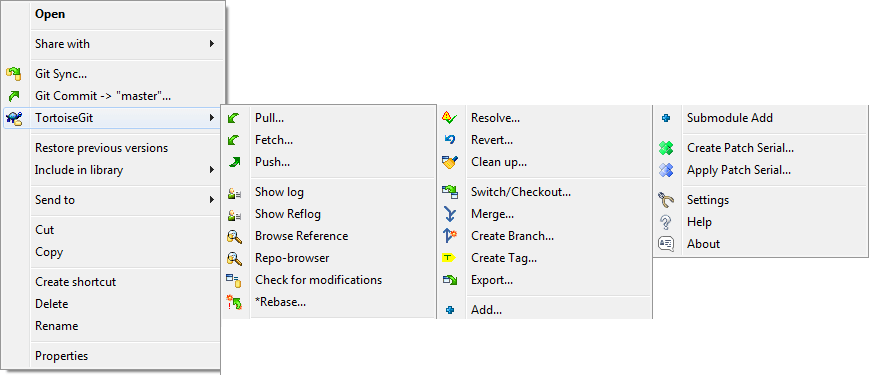
\includegraphics[width=\textwidth]{tg-ctx-wide.png}
		\caption{Affreux montage pour tout voir (c'est long)}
	\end{figure}
\end{frame}

\begin{frame}
	\frametitle{Installation}
	Deux composants sont nécessaires :
	\begin{itemize}
		\item Git (utilisable en ligne de commande)
			\begin{enumerate}
				\item \url{https://git-for-windows.github.io/}
				\item "Run Git from the Windows Command Prompt" %FIXME tester
				\item "Checkout Windows-style, commit Unix-style line endings"
			\end{enumerate}
			\pause
		\item TortoiseGit (l'interface, plus pratique) :
			\begin{enumerate}
				\item \url{https://tortoisegit.org/}, probablement x64
				\item Redémarrer (au moins logoff/logon) %FIXME?
			\end{enumerate}
	\end{itemize}
\end{frame}

\begin{frame}
	\frametitle{Au commencement...}
	Soit on part d'un dépôt existant (on le clonera à partir de GitHub,
	par exemple, voir slide \ref{f:gh}), soit on en crée un nouveau :
	\begin{itemize}
		\item Clic droit sur le dossier,
			\texttt{Git Create Repository Here}; \textit{ou}
		\item \texttt{git init} en console dans le dossier à gérer
	\end{itemize}

	Le dossier (\emph{dépôt}) est maintenant prêt à être versionné.
	\pause

	\begin{curieux}
		Un dossier caché \texttt{.git} vient d'apparaître
		\footnote{Pour ça, il faut que l'explorateur les affiche...}.
		Il contiendra toutes les versions (différentes) des fichiers.
	\end{curieux}
	\pause

	Plus de choses apparaissent dans le menu (cf. slide \ref{s:ctx})
\end{frame}

\begin{frame}
	\frametitle{Untracked, staged...}
	%TODO schéma ?
	Certains fichiers ne sont pas (encore ?) gérés, \texttt{untracked}.

	Les fichiers \texttt{staged} sont <<~en sécurité~>> :
	les changements ultérieurs peuvent être défaits
	à l'aide d'un \texttt{checkout} (cf. slide \ref{s:undo})
	mais ils ne sont pas encore repris dans l'historique
	(on ne peut donc pas encore les partager).
\end{frame}

\begin{frame}
	\frametitle{Créer ou modifier un fichier}
	Une fois que le fichier a été créé ou modifié, on peut le \emph{stage} :
	\begin{itemize}
		\item Clic droit sur le fichier, \texttt{Add}; \textit{ou} %FIXME?
		\item \texttt{git add f} en console dans le dossier où il se trouve
	\end{itemize}
\end{frame}

\begin{frame}
	\frametitle{Renommer/déplacer un fichier}
	Git n'est pas capable de voir de lui-même qu'un fichier a été déplacé (ou
	renommé, c'est idem). Il faut lui demander de le faire :
	\begin{itemize}
		\item Clic droit sur le fichier, \texttt{Rename}; \textit{ou} %FIXME?
		\item \texttt{git mv x y} en console dans le dossier où il se trouve
	\end{itemize}
\end{frame}

\begin{frame}
	\frametitle{Valider des changements}
	Une fois que les changements \texttt{staged} ont du sens ensemble,
	on peut les décrire dans le titre (et éventuellement le corps) d'un commit.
	Ils pourront ensuite être partagés avec les autres collaborateurs.
	\begin{itemize}
		\item Clic droit sur le fichier, \texttt{Commit}; \textit{ou} %FIXME?
		\item \texttt{git commit} en console
	\end{itemize}

	\begin{block}{Pour aller plus vite}
		On peut commit un fichier directement (\texttt{git commit x}).
	\end{block}

	\begin{block}{Quand on est allé trop vite}
		On peut commit un fichier par parties (\texttt{git add -p}).
	\end{block}
\end{frame}

\begin{frame}
	\frametitle{Voir l'historique}
	%FIXME fig
	\begin{itemize}
		\item Clic droit sur le dossier, \texttt{Show log}; \textit{ou} %FIXME??
		\item \texttt{git log} en console
	\end{itemize}
\end{frame}

\begin{frame}
	\frametitle{Défaire un changement}\label{s:undo}
	Plusieurs cas sont possibles :
	\begin{enumerate}
		\item Le fichier n'était pas versionné : dommage, il aurait dû l'être !
		\item Le changement n'a pas été \texttt{staged} :
			\begin{itemize}
				\item Clic droit sur le fichier, \texttt{Checkout}; \textit{ou} %FIXME??
				\item \texttt{git checkout f} en console
			\end{itemize}
		\item Le changement est dans un commit :
			\begin{itemize}
				\item S'il n'y a pas eu de \texttt{push}, %TODO amend ou rebase
				\item S'il a été partagé, %TODO revert (terminologie GUI ?)
			\end{itemize}
	\end{enumerate}
\end{frame}

\begin{frame}
	\frametitle{Qu'est-ce qui a changé depuis ce commit ?}
\end{frame}

\begin{frame}
	\frametitle{Qui a écrit cette merveille ?
	\footnote{Question alternative : c'est quoi cette m**** ?}}

	Il est parfois intéressant de voir qui a écrit une ligne dans un fichier.
	On pourrait le faire manuellement en parcourant l'historique mais ça peut
	vite devenir pénible et Git sait le faire tout seul :
	%FIXME fig

	\begin{itemize}
		\item Clic droit sur le fichier, \texttt{Blame}; \textit{ou} %FIXME?
		\item \texttt{git blame [--oneline] [--graph]} en console
	\end{itemize}
\end{frame}

\begin{frame}
	\frametitle{Débogage}
	Ça s'applique assez peu à un texte mais \texttt{git bisect} permet de
	déterminer quand un bogue est apparu (c'est plus facile quand on dispose de
	tests automatisés). Il suffit de lui indiquer un commit où ça fonctionnait
	et un autre où ce n'est plus le cas.

	Intuitivement, à chaque étape, il travaille par dichotomie.
	%FIXME script in fig
\end{frame}

\begin{frame}
	\frametitle{Branches}
	Nous avons jusqu'ici travaillé sur une seule branche. Il peut être utile de
	s'isoler (temporairement) pour travailler sur une partie, une fonctionnalité
	bien distincte; les branches permettent de le faire.
	%FIXME fig graph
	\begin{itemize}
		\item Clic droit, \texttt{Create Branch}; \textit{ou} %FIXME?
		\item \texttt{git checkout -b branche} en console permet de créer une
			branche et de passer dessus.
			La commande \texttt{git branch} affiche quant à elle celles
			qui existent\footnote{Localement...} et
			met en évidence celle sur laquelle on se trouve.
	\end{itemize}

	Si les fichiers ne sont ni modifiés, staged ou untracked, ils correspondent
	exactement à la la branche actuelle.
\end{frame}

\begin{frame}
	\frametitle{Merge (ou rebase puis merge ?)}
	Lorsque le résultat d'une branche peut être mis en commun, on peut le
	fusionner avec la branche principale (\texttt{master}) :
	\begin{itemize}
		\item Clic droit, \texttt{Merge}; \textit{ou} %FIXME?
		\item \texttt{git checkout master \&\& git merge branche} en console
	\end{itemize}

	Un \texttt{rebase} permet de rendre l'historique linéaire : Git va modifier
	les commits pour faire comme s'ils avaient été effectués après tous les
	changements de la branche cible.
	\begin{itemize}
		\item Clic droit, \texttt{Rebase}; \textit{ou} %FIXME?
		\item \texttt{git rebase master} puis merge (ci-dessus) en console
	\end{itemize}
\end{frame}

\begin{frame}
	\frametitle{GitHub}\label{f:gh}
	\begin{figure}[h]
		\centering
		\includegraphics{gh.png}
		\caption{Logo de GitHub}
	\end{figure}
	Cette plateforme héberge gratuitement des dépôts publics.

	Avec l'université
	\footnote{\url{https://education.github.com/discount_requests/new}},
	on dispose gratuitement de dépôts privés :
	ceux-ci ne seront visibles que par des personnes choisies.

	Pour pousser (si ça suit le dernier commit) :
	\begin{itemize}
		\item Clic droit, \texttt{Push...}; \textit{ou} %FIXME?
		\item \texttt{git push} en console
	\end{itemize}

	Pour tirer (fusion automatique) :
	\begin{itemize}
		\item Clic droit, \texttt{Pull...}; \textit{ou} %FIXME?
		\item \texttt{git pull} en console
	\end{itemize}

	\begin{curieux}
		Un merge équivaut à \texttt{git fetch && git merge}.
	\end{curieux}
\end{frame}


\end{document}
